
\textbf{Sensores}

Ao se expor todos os parâmetros de qualidade da água, é necessário se ter o conhecimento dos sensores que farão a
obtenção dessas informações. A seguir, se encontram uma série de sensores que foram pesquisados a fim de se ter uma 
idéia geral de quais equipamentos poderão ser utilizados no projeto. 

Sensores são dispositivos eletroeletrônicos que tem a propriedade de transformar em sinal elétrico a transformação
de uma grandeza física que esta relacionada a uma ou mais propriedade do material de que é feito o sensor. Esses elementos
são capazes de monitorar a variação de uma grandeza física e transmitir esta informação a um sistema em que a indicação
seja inteligível para nós ou para o elemento de controle do sistema. Os sensores são compostos por elementos denominados
transdutores que convertem uma grandeza de entrada em uma grandeza elétrica, que pode ser processada por um circuito
elétrico ou eletrônico \cite{vinay00}.

Existem diversos tipos de sensores os que julgamos necessários para o controle do sistema de capitação de água pela rotação
da turbina. São os sensores de umidade relativa do ar, sensores de velocidade e direção do vento (anemômetro), sensores
de nível e fluxo de entrada e saída de água, sensores de oxigênio, sensores de condutividade, sensores de pH, sensores
de turbidez, sensores de nitrato/nitrogênio, entre outros.

  \begin{enumerate}
  
    \item \textbf{Sensor da umidade do ar e temperatura}
      
	Características:
	
	\begin{itemize}
	 \item Processamento digital de sinal
	 \item Umidade relativa e temperatura do ar em um único sensor
	 \item Alta acurácia de leitura e linearização
	 \item Sinais de saída condicionados
	 \item Excelente estabilidade de longo termo
	 \item Baixo tempo de resposta
	 \item 100\% intercambialidade
	\end{itemize}

	Construção:
	
	O invólucro do sensor e do circuito eletrônico é moldado em plástico injetado e estabilizado para U.V.
	O invólucro do circuito é selado, sendo à prova de respingos e poeira. Todas as conexões elétricas
	são feitas através de um conector selado na base do sensor. O sensor opera de 0 a 100\% umidade relativa.
	Os transdutores internos não sofrem danos mesmo com condensação. O circuito digital do sensor realiza a
	compensação de temperatura e a linearização do sinal de saída. O armazenamento dos dados de calibração do
	 sensor em memória interna não volátil fornece uma maior acurácia nas leituras.
	 
	 \begin{figure}[!htbp]
	  \centering
	  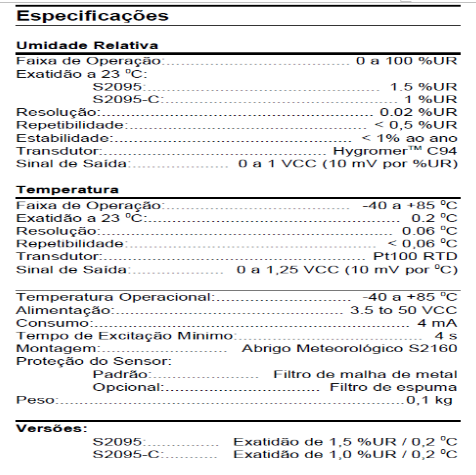
\includegraphics[scale=0.5]{editaveis/figuras/especificacao_sensor_umidade}
	  \caption[Especificação do sensor de umidade e temperatura]{Especificação do sensor de umidade e temperatura. \footnotemark}
	  \FloatBarrier
	  \label{especificacao_sensor_umidade}
	 \end{figure}
	 \footnotetext{Fonte: \cite{squitter}}
	 
    \item \textbf{Sensor de pH}
    
	O sensor de pH da água é de extrema importância para o projeto da “planta de abastecimento de água potável
	através da umidade do ar” pois monitora um dos índices de qualidade da água especificados pela \cite{anaGov}.
	
	\begin{center}
	 \textbf{Especificação do sensor de pH}
	\end{center}

	Para aplicações industriais, o método de medição de pH mais empregado é o eletrodo de vidro \cite{sole79}.
	Os eletrodos de pH possuem basicamente o mesmo funcionamento que as baterias: transferem uma tensão mínima que poderá
	ser detectada por um medidor ou um regulador de pH. A diferença é que os eletrodos de pH não produzem tensão de forma
	contínua, a não ser quando são introduzidos num líquido.
	
	\begin{center}
	 \textbf{Calibração de sensores de pH}
	\end{center}
	
	O período de calibração de um sensor de pH depende do contexto em que o sensor será aplicado e do tipo de sensor
	que será utilizado. O tipo de sensor a ser utilizado pode variar de acordo com parâmetros como temperatura.
	O sensor de pH pode vir acoplado a um sensor de condutividade, entre outros. Apesar de existirem vários tipos,
	todo eletrodo de pH requer calibração periódica. Uma calibração em dois pontos caracteriza um eletrodo com um
	medidor de pH específico. Uma desvantagem dos sensores de pH é que eles necessitam de calibração diária.
	Neste caso, seria necessário um funcionário que realizasse a calibração diariamente, ou de um sistema automatizado
	que realize a calibração.
	
	
    \item \textbf{Sensor ORP}
    
	O sensor ORP é similar ao sensor pH quanto ao seu funcionamento, porém, ao invés de seu eletrodo ser envolvido por
	vidro, é geralmente envolvido por platina ou ouro, devido ao fato de esses metais não interferirem nas reações químicas.
	Nos sensores ORP, o gel interno recebe a corrente elétrica provinda do meio e a transmite ao interior do sensor.
	Posteriormente, o fio e prata pura transmite a corrente positiva ao para o cabo de conexão, que leva o sinal recebido
	ao controlador.
	
    \item \textbf{Sensor de turbidez}
    
	Os sensores de turbidez são necessários para aferir a quantidade de sólidos que existem na água, já que este é um dos
	índices de qualidade da água definidos pela ANA.
	
	\begin{center}
	 \textbf{Especificação do sensor de turbidez}
	\end{center}
	
	O sensor de turbidez é o equipamento utilizado para medir a turbidez de um líquido. A aferição compara o espalhamento
	de um feixe de luz ao passar pela amostra, com o de um feixe de igual intensidade, ao passar por uma suspensão
	padrão \cite{usepa99}. Os sensores de turbidez funcionam por meio de detectores fotoelétricos, que são sensíveis
	a sutis mudanças na intensidade da luz, proporcionando uma maior precisão. O sensor de turbidez utilizado
	atualmente é o turbidímetro nefelométrico. 
	
	\begin{center}
	 \textbf{Funcionamento do sensor de turbidez}
	\end{center}
	
	O princípio de funcionamento dos turbidímetros atuais, baseia-se na emissão de um feixe luminoso e na detecção da luz
	refletida pelas partículas em suspensão ou diferença de intensidade entre a luz emitida e recebida, a qual é convertida
	em sinal elétrico e mostrada no equipamento. Nos instrumentos comerciais o detector é disposto em ângulos de
	45, 90 ou 180 graus. A emissão de luz normalmente é obtida por meio de lâmpadas de mercúrio,lâmpadas de tungstênio,
	laser ou diodos de emissão \cite{padua06}. Os sensores de turbidez processam as informações analógicas 
	e as devolvem em forma de tensão.
	
	\begin{center}
	 \textbf{Calibração do sensor de turbidez}
	\end{center}
	
	A calibração do sensor de turbidez pode ser feita de três formas:
	
	\textbf{Calibração direta} na qual é utilizada uma solução padrão de formazina para a calibração do sensor.
	\textbf{Calibração Indireta} na qual a grandeza que deseja ser medida é fornecida por um meio externo, como um equipamento
	  previamente calibrado, que atua simultaneamente no Sistema de Medição em Calibração e no Sistema de Medição Padrão,
	  e é feita uma comparação com os resultados obtidos \cite{cni01}.
	\textbf{Via Software} na qual a calibração é feita por um software que pode ser realizada no próprio aparelho ou com a
	  utilização de um computador que faz a calibração quando o sensor é conectado. 
	
    \item \textbf{Sensor de temperatura da água}
	
	Os sensores de temperatura da água medem a temperatura da água e funcionam segundo o princípio de resistência variável.
	Os sensores de temperatura de líquidos em geral são envolvidos por materiais com alta resistência a corrosão.
	Estes sensores funcionam com transdutores, que são componentes que possuem a função de transformar grandezas elétricas.
	Basicamente, um sensor de temperatura é uma espécie de resistor que aumenta sua resistência quando a temperatura do
	líquido aumenta.
	
    \item \textbf{Sensor de temperatura da água}
	
	\begin{center}
	 \textbf{Calibração do sensor de temperatura da água}
	\end{center}
	
	Uma das vantagens dos sensores de temperatura é o fato de que estes componentes não necessitam de calibração constante.
	Um dos métodos de calibração mais utilizados atualmente é o Método Comparativo no qual o sensor a calibrar tem sua
	indicação comparada com as de um padrão de referência. O método consiste em imergir ambos em um meio térmico uniforme
	e estável, cuja temperatura possa ser controlada na faixa requerida.
	
    \item \textbf{Sensor de nitrogênio}
	 
	O Nitrogênio pode ser encontrado no meio aquático nas seguintes formas: nitrogênio molecular, nitrogênio orgânico,
	nitrogênio amoniacal (amônia), nitrato e nitrito. Na natureza o nitrogênio está presente nas proteínas e pode advir
	também da composição celular de microorganismos. Quanto à origem antropogênica do nitrogênio pode ser proveniente 
	também de despejos domésticos e industriais assim como de excrementos animais e fertilizantes químicos, podendo indicar
	grau de contaminação \cite{sperling96}. A falta de controle do nível de nitrogênio pode acarretar danos nos 
	filamentos das brânquias e diminuição imunológica levando-o a morte.
	
	O aparelho que será utilizado para medição do nível de nitrogênio é a sonda YSI 6820 V2.
	
	\begin{table}[h]
	\centering
	\begin{tabular}{|c|c|p{6cm}|p{5cm}|}
	
	\hline
	Nitrato/Nitrogênio &
	0 a 200 mg/L-N &
	0,001 a 1 mg/L(em função da faixa de leitura) &
	10\% da leitura ou 2mg/L, o que for maior.\\
	\hline

	\end{tabular}
	\end{table}
    
    \item \textbf{Sensor de oxigênio dissolvido}
    
	O nível de oxigênio dissolvido na água é o parâmetro mais importante especificado pela ANA,
	para medir-se este parâmetro em tempo real, utiliza-se um sensor, chamado de sensor eletroquímico
	de oxigênio dissolvido.
	
	Esse sensor possui no seu interior uma membrana permeável ao gás que envolve um eletrodo que reage com
	o oxigênio dissolvido, quando a quantidade de oxigênio cai, o catodo gera uma corrente proporcional à
	pressão exterior a membrana \cite{ferreira07}.
	
	\begin{figure}[!h]
	  \centering
	  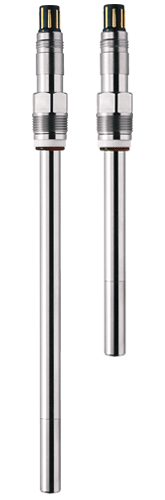
\includegraphics[scale=0.4]{editaveis/figuras/sensor_oxigenio}
	  \caption[Sensor de oxigênio dissolvido]{Sensor de oxigênio dissolvido}
	  \FloatBarrier
	  \label{sensor_oxigenio}
	 \end{figure}
	
	\begin{center}
	 \textbf{Medição de nível de fosforo total}
	\end{center}
	
	O fosforo encontrado na agua pode ter origem da dissolução doas solos e decomposição de matéria orgânica,
	do uso de fertilizantes, despejos domésticos e industriais, detergentes e excrementos animais \cite{danelon12}.
	
	Então é importante que os níveis do fosforo sejam controlados, seguindo os níveis propostos pela ANA,
	para medir-se esse parâmetro, não é possível por meio de sensores, então
	se utiliza um aparelho chamado de Fotômetro medidor de fósforo.
	
    \item \textbf{Coliformes fecais}
    
	Coliformes totais são bactérias que não causam doenças, uma vez que habitam o intestino de animais mamíferos inclusive
	o homem. Dentre as bactérias pertencentes ao grupo coliforme totais, a mais estudada é a \textit{Escherichia Coli} (E. Coli),
	resumida como pertencente ao grupo das enterobacterias \cite{neidhardt96}.
	
	A determinação da concentração dos coliformes assume importância como parâmetro indicador da possibilidade da 
	existência de microorganismos patogênicos, responsáveis pela transmissão de doenças de veiculação hídrica, tais como
	febre tifóide, febre paratifóide, desinteria bacilar e cólera \cite{anaGovIndicadores}.
	
	A importância dos coliformes também está relacionada com a qualidade da água, uma vez que é um dos principais
	parâmetros para o cálculo do Índice de Qualidade de Água (IQA) \cite{cetesbIndiceQualidadeH2O}.
	
	A análise de coliformes deve ser realizada de acordo com as normas técnicas da CETESB que prescrevem que a análise
	deve ser realizada por meio da técnica de membrana filtrante para determinação da densidade de bactérias do grupo
	coliforme, com aplicação em: controle de qualidade de águas destinadas: ao abastecimento público (sem ou com simples
	desinfecção, ou após tratamento simplificado ou convencional); a irrigação de hortaliças e plantas; a recreação de
	contato primário (natação, esqui-aquático, mergulho); a criação natural e/ou Anais XVI Simpósio Brasileiro de
	Sensoriamento Remoto - SBSR, Foz do Iguaçu, PR, Brasil, 13 a 18 de abril de 2013, INPE 6652 intensiva (aquicultura)
	de espécies destinadas a alimentação humana; a dessedentarão de animais; ao abastecimento industrial \cite{cetesb84}.
	
	A quantidade de coliformes fecais não deve exceder um limite de 200 por 100 mililitros em 80\% ou mais de pelo menos
	5 amostras mensais colhidas em qualquer mês.
	
  \end{enumerate}
